In this section we present our main results for the detectable LISA DCO population. We find that on average, for our fiducial model, a 4-year LISA mission will detect about \BHBHFourYear{} BHBHs, \BHNSFourYear{} BHNSs and \NSNSFourYear{} NSNSs (c.f.\ Table~\ref{tab:detection_rates}). We first show the distribution of the sources together with the sensitivity curve in Section~\ref{sec:dcos_on_sc}, before exploring the variations in the detection rate over different physics variations in Section~\ref{sec:detection_rate_analysis} and analysing the parameter distributions for detectable sources in the fiducial model in Section~\ref{sec:fiducial_distributions}.

\subsection{Distribution on the sensitivity curve}\label{sec:dcos_on_sc}

\begin{figure*}[tp]
    \centering
    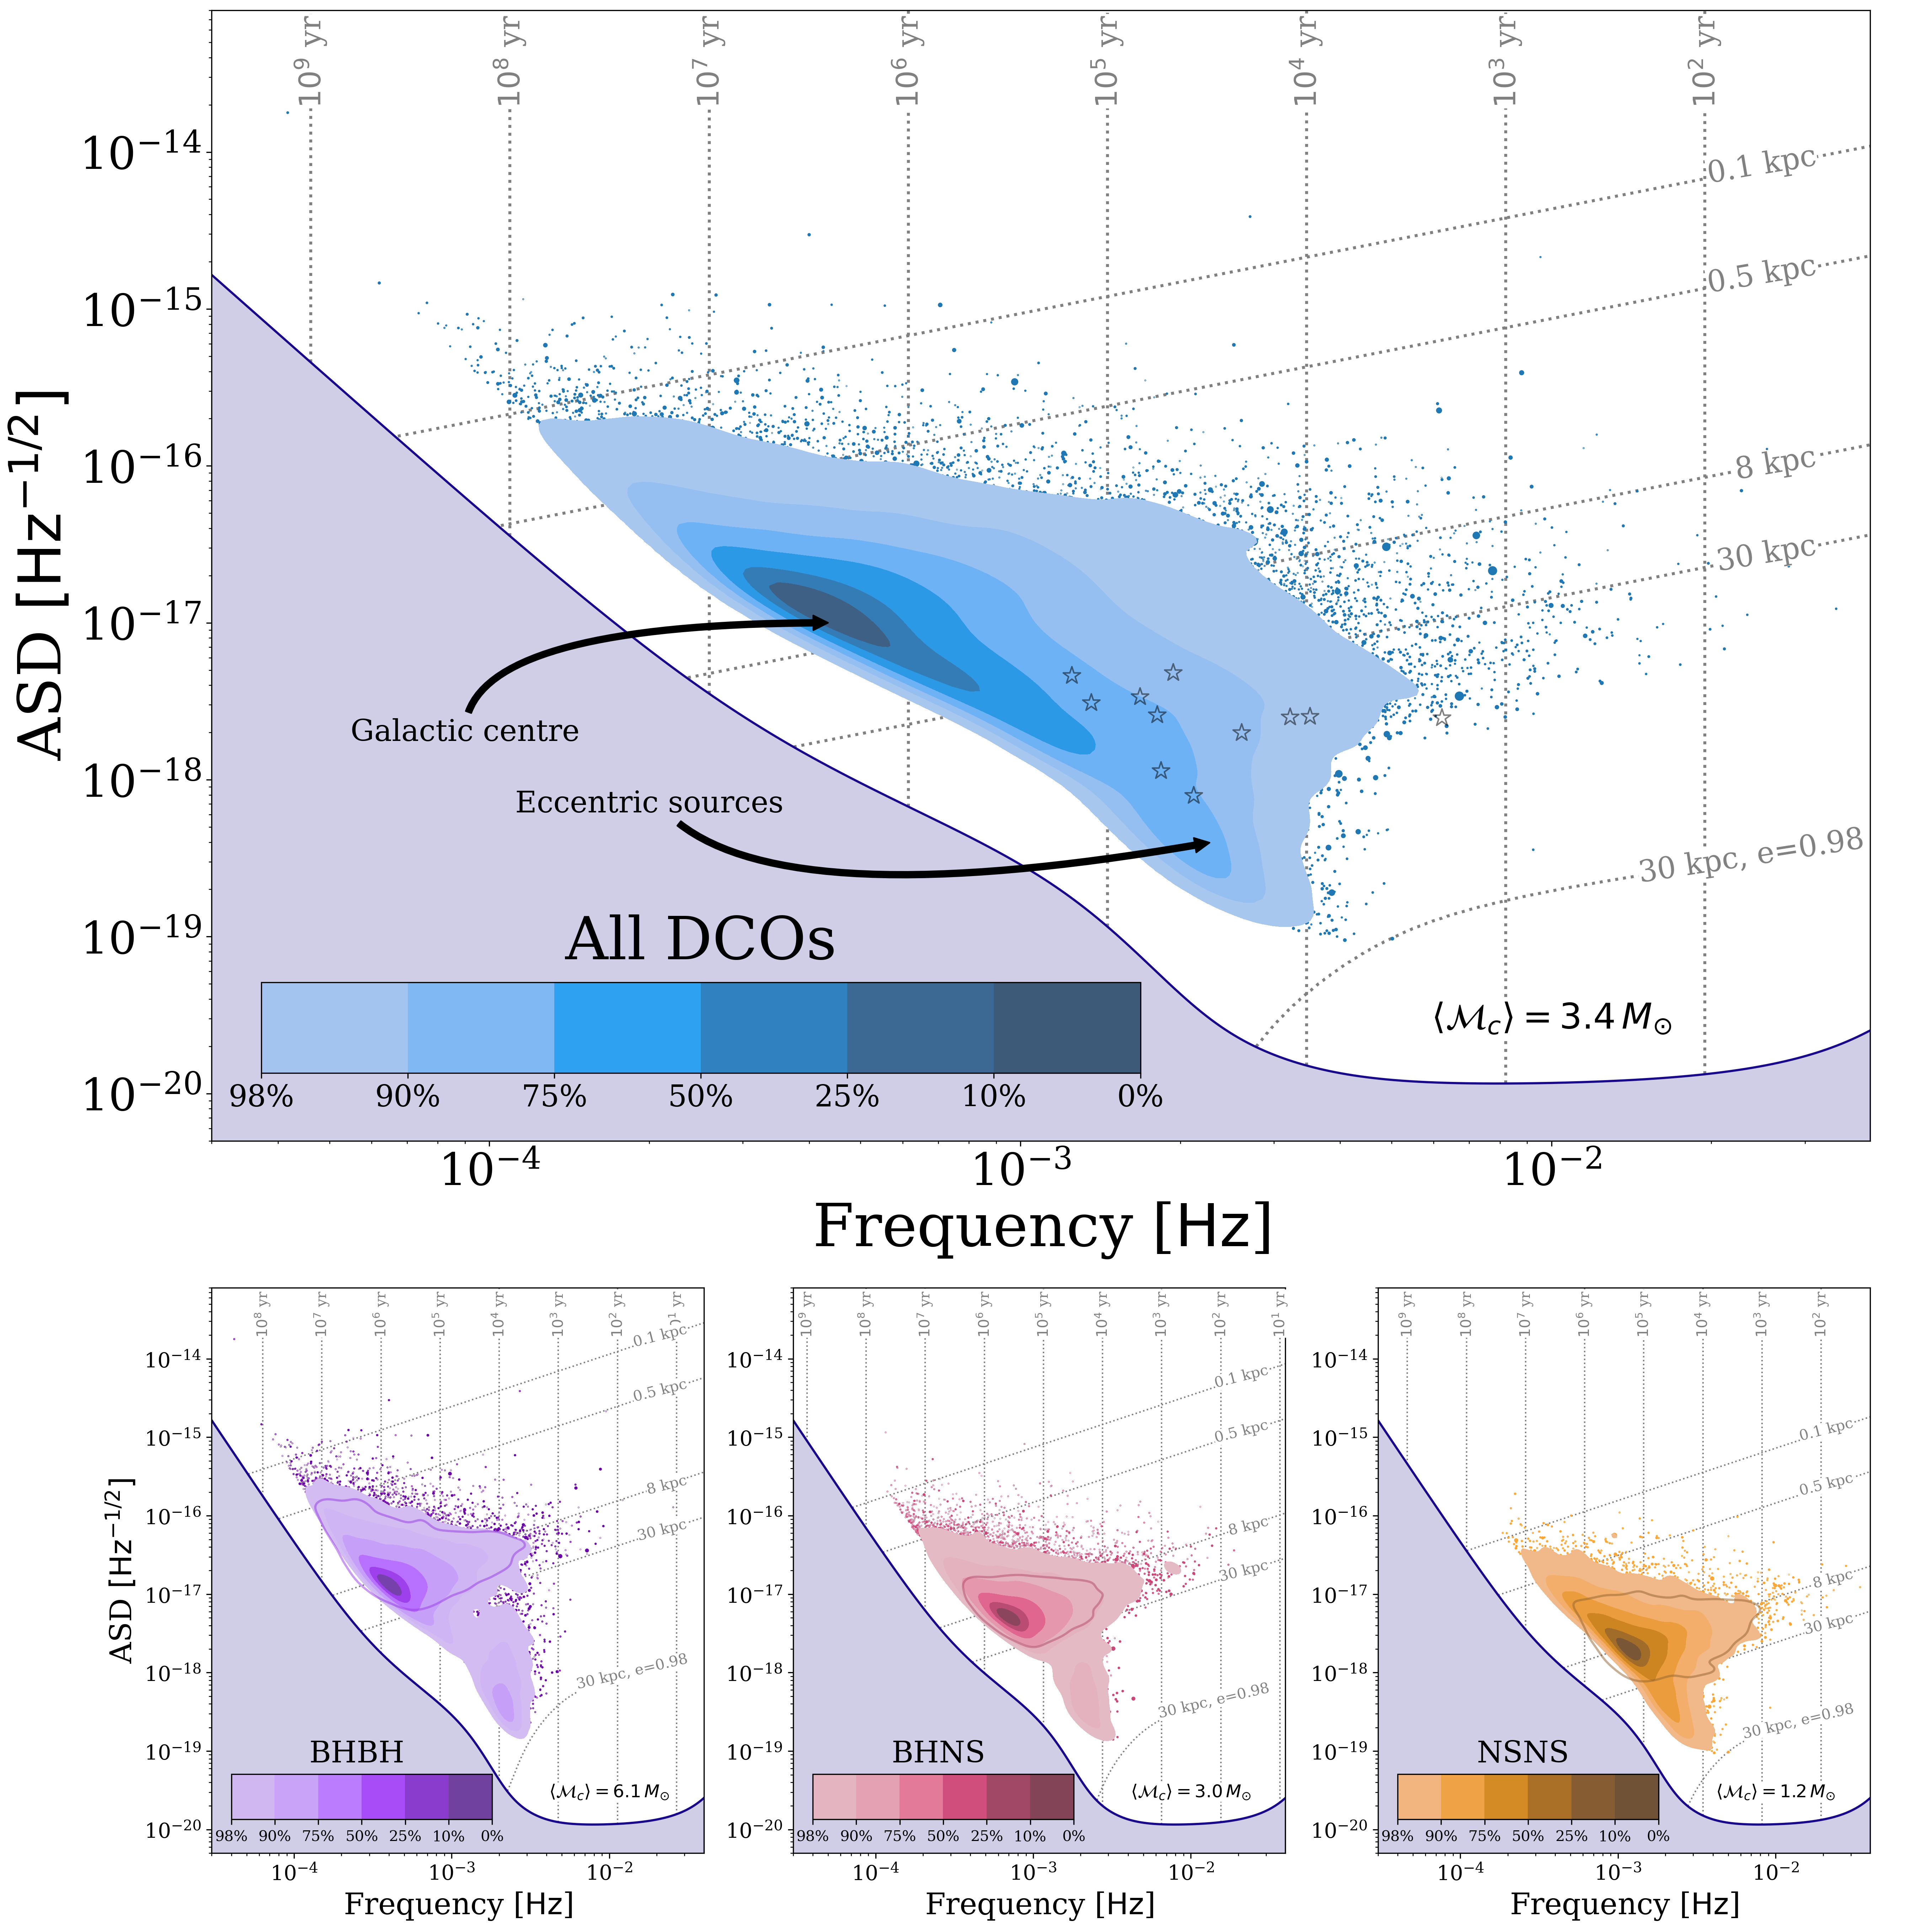
\includegraphics[width=\textwidth]{2_dcos_on_sc.png}
    \caption{Density distribution of detectable BHBH, BHNS and NSNS binaries are shown together with the LISA sensitivity curve. In the top panel we show all systems with the LISA verification binaries over plotted (star symbols, \citealp{Kupfer+2018}). In the bottom panels we separate by type. Contours show the percentage of the population enclosed. The remaining 2\% of the population is shown as dots with a size that scales with the sampling weight. For reference we show lines where a circular binary of average mass $\avg{\mathcal{M}_c}$ would reside for a given remaining inspiral time (vertical lines) and distance (diagonal line). To highlight the role of eccentricity we further show the signal expected for an eccentric binary at 30 kpc. The coloured line in the bottom panels shows a contour that encloses 90\% of the population that is circular. See Sec.~\ref{sec:dcos_on_sc} for a discussion.}
    \label{fig:dcos_on_sc}
\end{figure*}

We show the expected distribution of detectable DCOs together with the LISA sensitivity curve in Figure~\ref{fig:dcos_on_sc}. This shows that the detectable population of these massive DCOs is concentrated at comparatively lower frequencies than the LISA verification binaries (shown as stars in the top panel). This is expected since producing the same SNR as a BHBH, BHNS or NSNS with a relatively lower mass (circular) WDWD requires a higher frequency. This finding is in agreement with \citet{Sesana+2020} and as noted in that work, this could possibly be used to distinguish these more massive DCOs from WDWDs probabilistically. There are several other notable features in these distributions and to understand these we overplot reference lines indicating where a circular binary with the average chirp mass (annotated in each panel) would reside for a given remaining inspiral time (vertical lines) and a given distance (diagonal lines).

We would expect that if a population was entirely circular, it should be bounded approximately between the $0.1$--$30 \unit{kpc}$ lines (roughly the minimum and maximum distance to a source in the Milky Way). From inspection of the bottom panels with each individual DCO type we see that, though this is the true for a large fraction of the population, there is a distinct subpopulation of binaries that extend downwards, especially around $2 \unit{mHz}$. This offshoot is composed of eccentric binaries for which the circular distance contours do not apply. For instance, we plot the 90\% contour of only the circular sources in our sample over the density distribution in each of the bottom panels and it is clear that the circular subsample is bounded by the distance lines. We also plot a line of constant distance at $30 \unit{kpc}$ for an eccentric binary with $e = 0.98$ to show the differences for eccentric sources. Additionally, we note that the peak of the density distribution coincides with the centre of the Milky Way as expected, since binaries are most likely to be formed towards the centre of the Galaxy.

We plot vertical lines that give the inspiral time for a circular binary with the average chirp mass (annotated in each panel). From these lines we can understand the trend of the density distribution decreasing with increasing frequency. Sources with higher frequencies have shorter inspiral times and thus DCOs will spend less time in these regimes, meaning that more sources are detected at lower frequencies. Note that these inspiral time lines should only be used as guidelines for the population as a whole, as the inspiral time of each individual source will be a function of its mass and eccentricity. It is also evident for each DCO source that the tail of the high frequency sources is more numerous near to the Galactic centre than at short distances. This is simply because there are more sources in the galactic centre and so the chances of `catching' a binary at high frequency are better.

\subsection{Detection rates}\label{sec:detection_rate_analysis}
\tom{I will be updating this section once the other physics variations are done running. There will be a couple of new models and the current ones will have better high Z resolution.}
We find that for our fiducial model on average, a 4-year LISA mission will detect \BHBHFourYear{} BHBHs, \BHNSFourYear{} BHNSs and \NSNSFourYear{} NSNSs. Increasing to a 10-year LISA mission length changes the number of detections to \BHBHTenYear{}, \BHNSTenYear{} and \NSNSTenYear{} respectively. In Figure~\ref{fig:detection_rates}, we show the expected number of LISA detections for each model variation and discuss the prominent trends in the following sections. We show the rates and uncertainties plotted in this figure in Table~\ref{tab:detection_rates}.

\begin{figure*}[p]
    \centering
    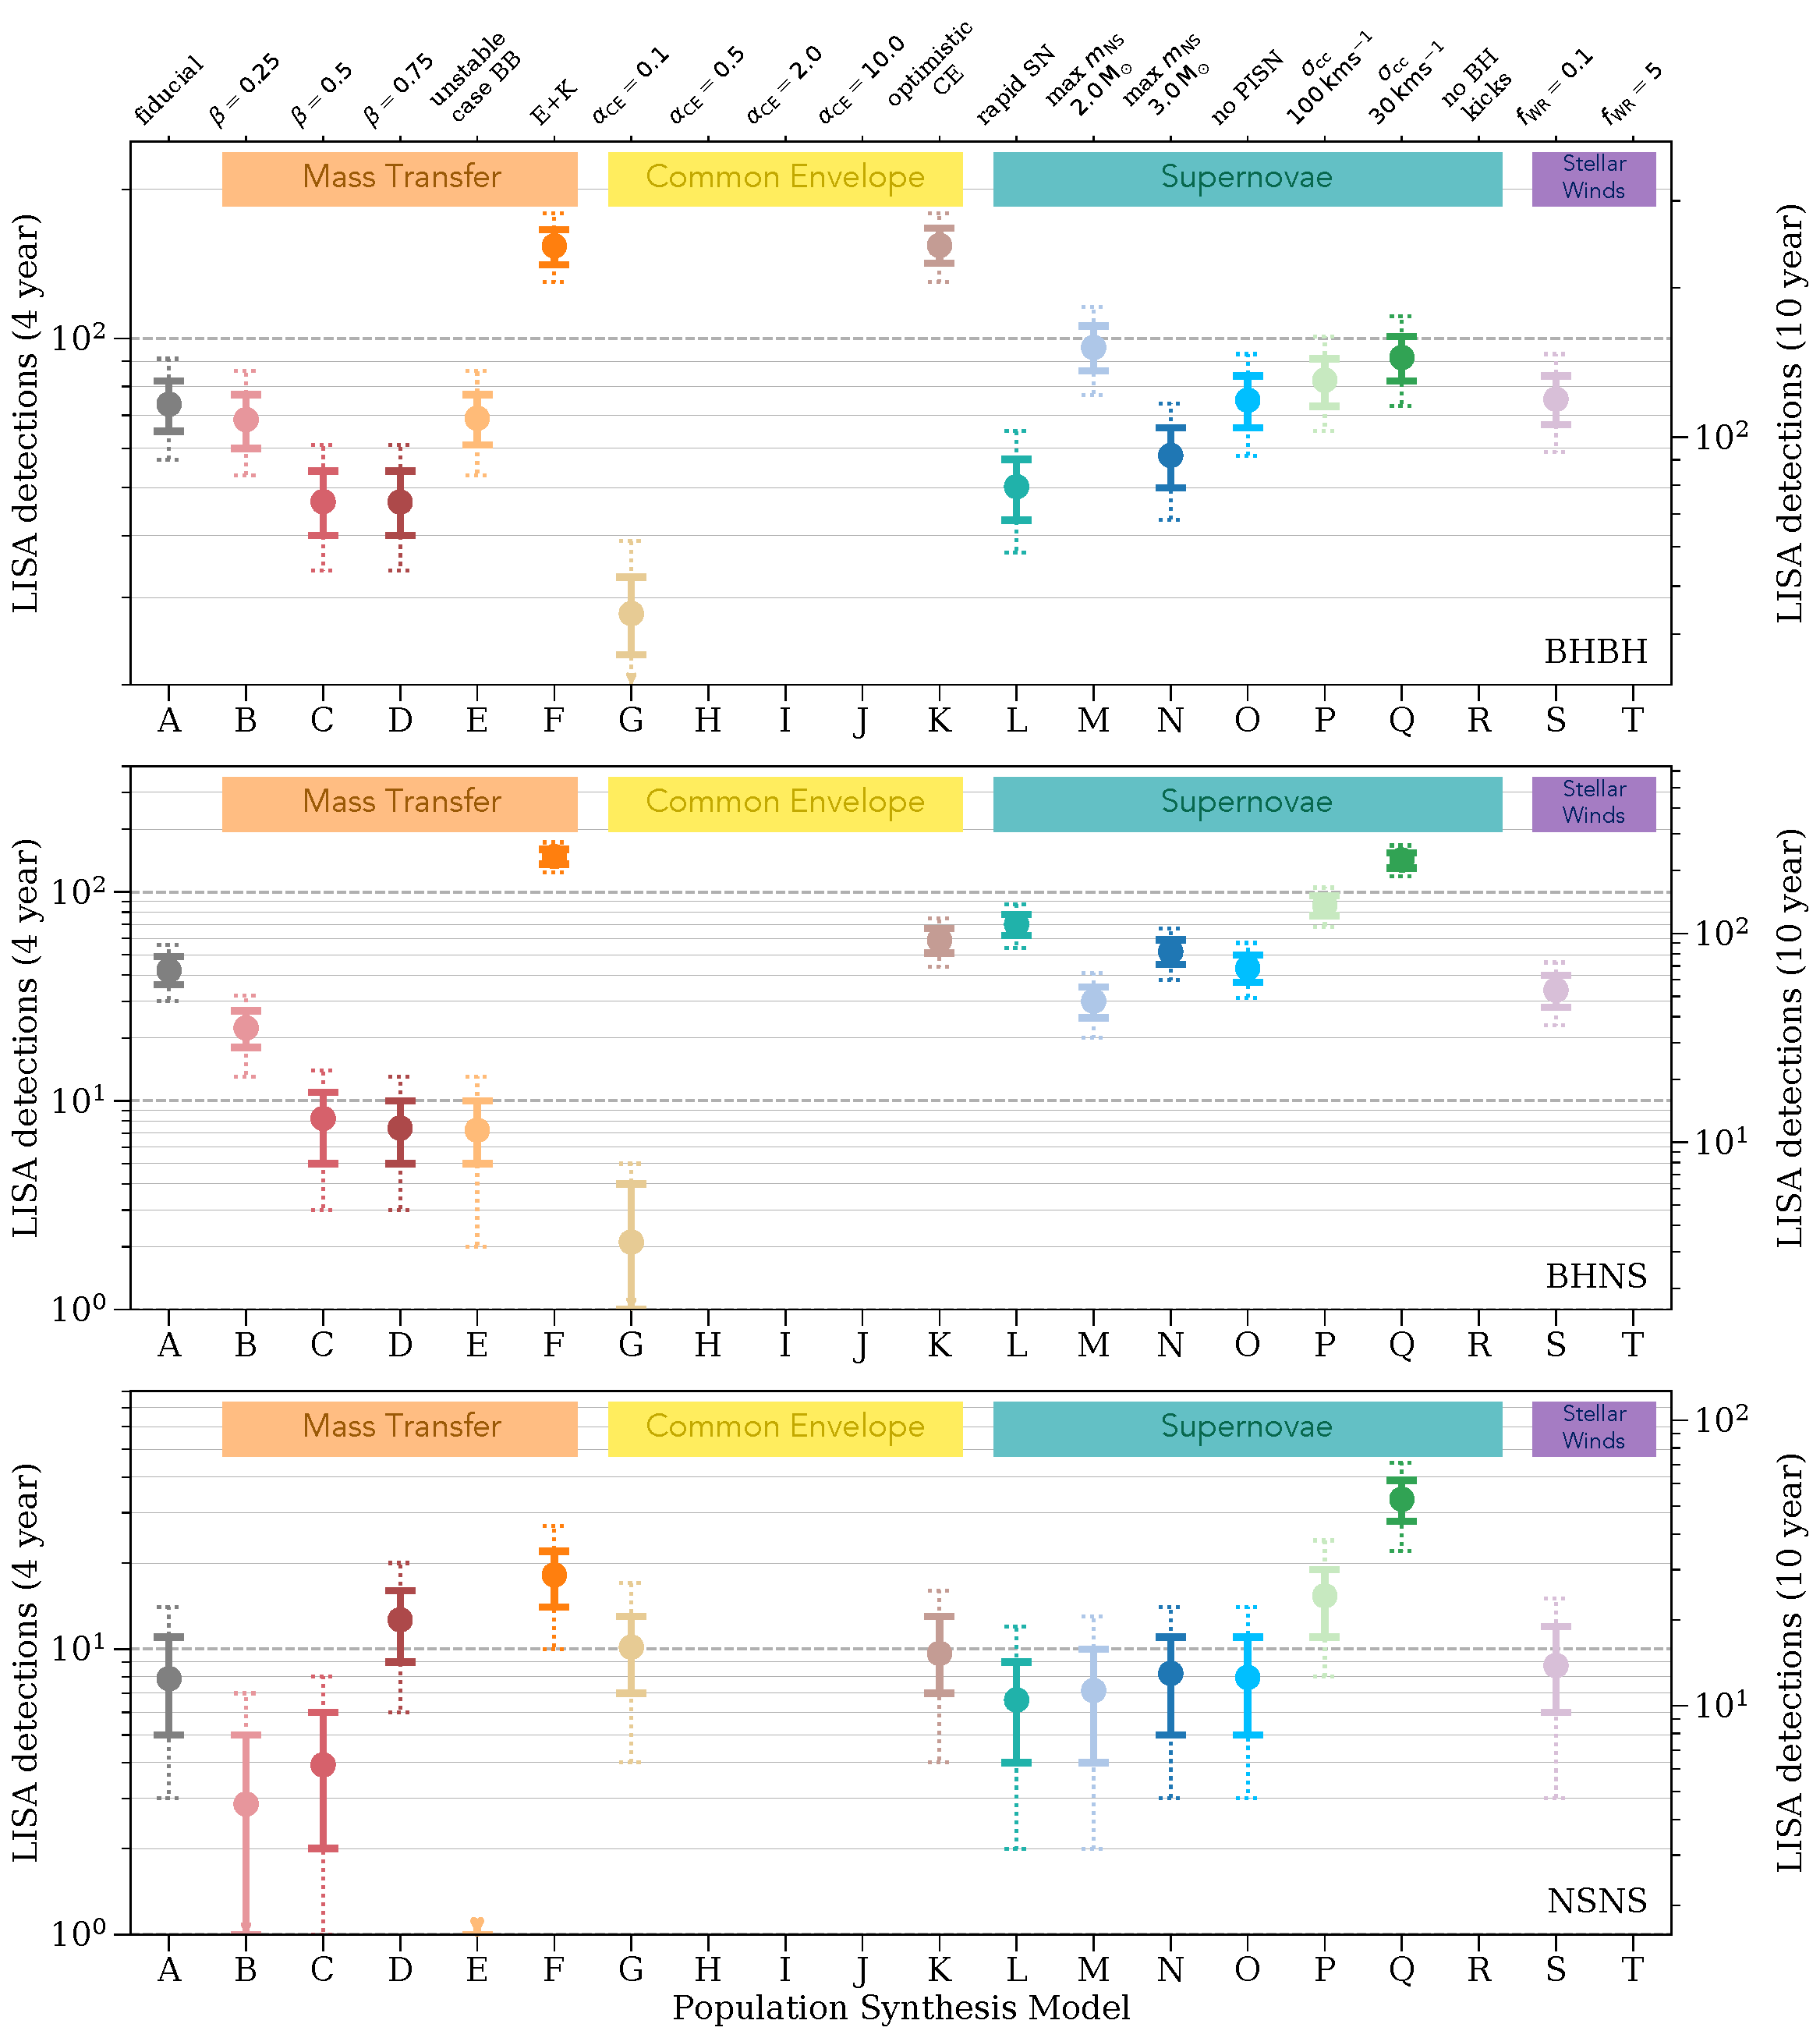
\includegraphics[width=\textwidth]{3_dco_detections.pdf}
    \caption{The number of expected detections in the LISA mission for different DCO types and model variations. Error bars show the 1- (solid) and 2-$\sigma$ (dotted) Poisson uncertainties. An arrow indicates that the error bar extends to zero. The left axis and grid lines show the number of detections in a 4-year LISA mission and the right axis shows an approximation of the number of detections in a 10-year mission (we scale the axis by $\sqrt{T_{\rm obs}}$, see Table~\ref{tab:detection_rates} for exact rates). Each model is described in further detail in Table~\ref{tab:physics_variations} and details of the fiducial assumptions are in Section~\ref{sec:fiducial_physics}. \todo{subject to change with the updated/new models and new uncertainty estimates}}
    \label{fig:detection_rates}
\end{figure*}

\subsubsection{BHBH detection rate trends}
The BHBH detection rate is markedly robust across physics variations, with the expected detections in each model staying within 25\% of the fiducial rate (with the exception of model \modOpt{}). Thus even if there are changes in our understanding of the underlying physics before the LISA mission commences, the expected BHBH detection rate is unlikely to change significantly.

The exception to this statement is model \modOpt{}, in which we allow Hertzsprung gap donors to survive common envelope events. A large fraction of the progenitors of BHs in this mass range expand significantly during the Hertzsprung gap phase and initiate common envelope events. Therefore, though the detectable fraction does not change significantly, the increased population of BHBHs in the Milky Way leads to this model predicting 2.5 times more detections.

\subsubsection{BHNS detection rate trends}
In contrast, the BHNS detection rate is very sensitive to changes in binary physics assumptions. Therefore, once LISA flies and we know the actual number of detections, we can compare to each model and possibly provide some constraint on binary evolution physics. There are several notable trends in the BHNS detection rate in the middle pane of Figure~\ref{fig:detection_rates}.

As $\beta$ increases in models \modBetaLow{}-\modBetaHigh{}, the BHNS detection rate steadily decreases. This may seem unintuitive since a higher mass transfer efficiency should lead to more massive compact objects and thus a more detectable population. However, one must also consider that most of these DCOs are formed through a common envelope event and so retaining more of the envelope during mass transfer means that the eventual ejection of the envelope is much more difficult, thus leading to more stellar mergers and fewer detectable BHNSs \citep[e.g.][]{Kruckow+2018}.

\tom{@ALL, the trend with common envelopes still confuses me, specifially, why does it not increase when $\alpha=2.0$? We never quite resolved this in the thread in zpro\_tom\_wagg with me and Lieke. I do see that the BHBH have a lot of only stable mass transfer and so reasonably are not too affected. NSNS basically only come through CE events and so sensibly are strongly affected but BHNS have $\sim 70\%$ classic channel and so should be affected strongly. But we don't see an increase with $\alpha = 2.0$. Any thoughts? (I'm leaving thinking about this for now in case it changes with the new data haha)}
% For a similar reason, the rate is decreased when $\alpha$ is decreased in model \modAlphaLow{}, as this reduces the amount of orbital energy that is used to eject the envelope and thus leads to more stellar mergers. \todo{Why isn't the opposite true for model \modAlphaHigh{}? It seems the number of bound DCOs \textit{does} increase but the merging total decreases...?}

Enforcing that case BB mass transfer is always unstable (model \modCaseBB{}) decreases the detection rate as fewer NSs are produced and thus fewer BHNSs form. This is explained in further detail in Section~\ref{sec:NSNS_detection_trends}. For the same reason as the BHBH rate, model \modOpt{} has a higher number of detections. This change is less prominent than in the BHBH case as the progenitors tend to be lower masses and initiate a CE event less frequently during the Hertzsprung gap phase. 

The Fryer \textit{rapid} prescription (model \modRapid{}) leads to a higher detection rate for BHNSs because progenitors that would become black holes in the \textit{delayed} prescription, instead become neutron stars and so more BHNSs are formed instead of BHBHs. For the same reason, increasing the maximum neutron star mass (model \modNSHigh{}) increases the detection rate and the inverse is true when it is decreased (model \modNSLow{}).

Finally, models \modSigLow{}-\modNoBH{} show increased detection rates since lower kicks result in fewer disrupted binaries and hence a more numerous detectable population. Following this logic it makes sense that model \modSigLower{} produces more detections than model \modSigLow{}. The model with no BH kick (\modNoBH{}) is slightly lower than model \modSigLower{} as the number of surviving binaries is limited by the neutron star kick more than the black hole kick.

\subsubsection{NSNS detection rate trends}\label{sec:NSNS_detection_trends}

As $\beta$ increases the NSNS detection rate increases, the opposite trend to that seen in the BHNS rate. This is for two main reasons: firstly the ejection of a common envelope is less problematic for the less massive NSNS binaries. Moreover, the increased mass transfer efficiency means that systems that were previously below the mass necessary to become a NS can now accrete enough mass to form a NS. Although the same is true for more massive stars becoming BHs instead of NSs, due to the IMF, there is a net flux of more stars becoming NSs.

There is a drastic decrease in detections for model \modCaseBB{} by nearly two orders of magnitude. This is because the majority of NSNS binaries are formed through case BB mass transfer and setting this mass transfer to be always unstable results in many of these binaries to merge before they could become NSNSs. As a result the total number of detections decreases, however, interestingly the remaining population represent more massive progenitors (that would not go through case BB mass transfer) and thus is skewed to higher masses and has a \textit{higher} detectable fraction.

The vast majority of NSNSs in our sample are formed through the common envelope channel and thus changing the value of $\alpha_{\rm CE}$ has an effect on the rate. We see that decreasing $\alpha_{\rm CE}$ (model \modAlphaLow) leads to a lower rate as there is less energy available to eject the envelope and so more binaries result to stellar mergers rather than NSNSs and similarly we see an inverse trend when increasing $\alpha_{\rm CE}$ (model \modAlphaHigh).

As we found in the BHNS trends, a lower value for the core-collapse supernova velocity dispersion increases the detection rate in models \modSigLow{} and \modSigLower{}, whilst changing the PISN or BH kick prescription (models \modNoPISN{} and \modNoBH{}) of course has no effect on the NSNS population.

\subsection{Properties of the detectable systems}\label{sec:fiducial_distributions}

In Figure~\ref{fig:fiducial_pdf_distributions}, we show the distribution of the individual parameters of the population of detectable binaries and discuss the various features in the following sections.

\begin{figure*}[htbp]
    \centering
    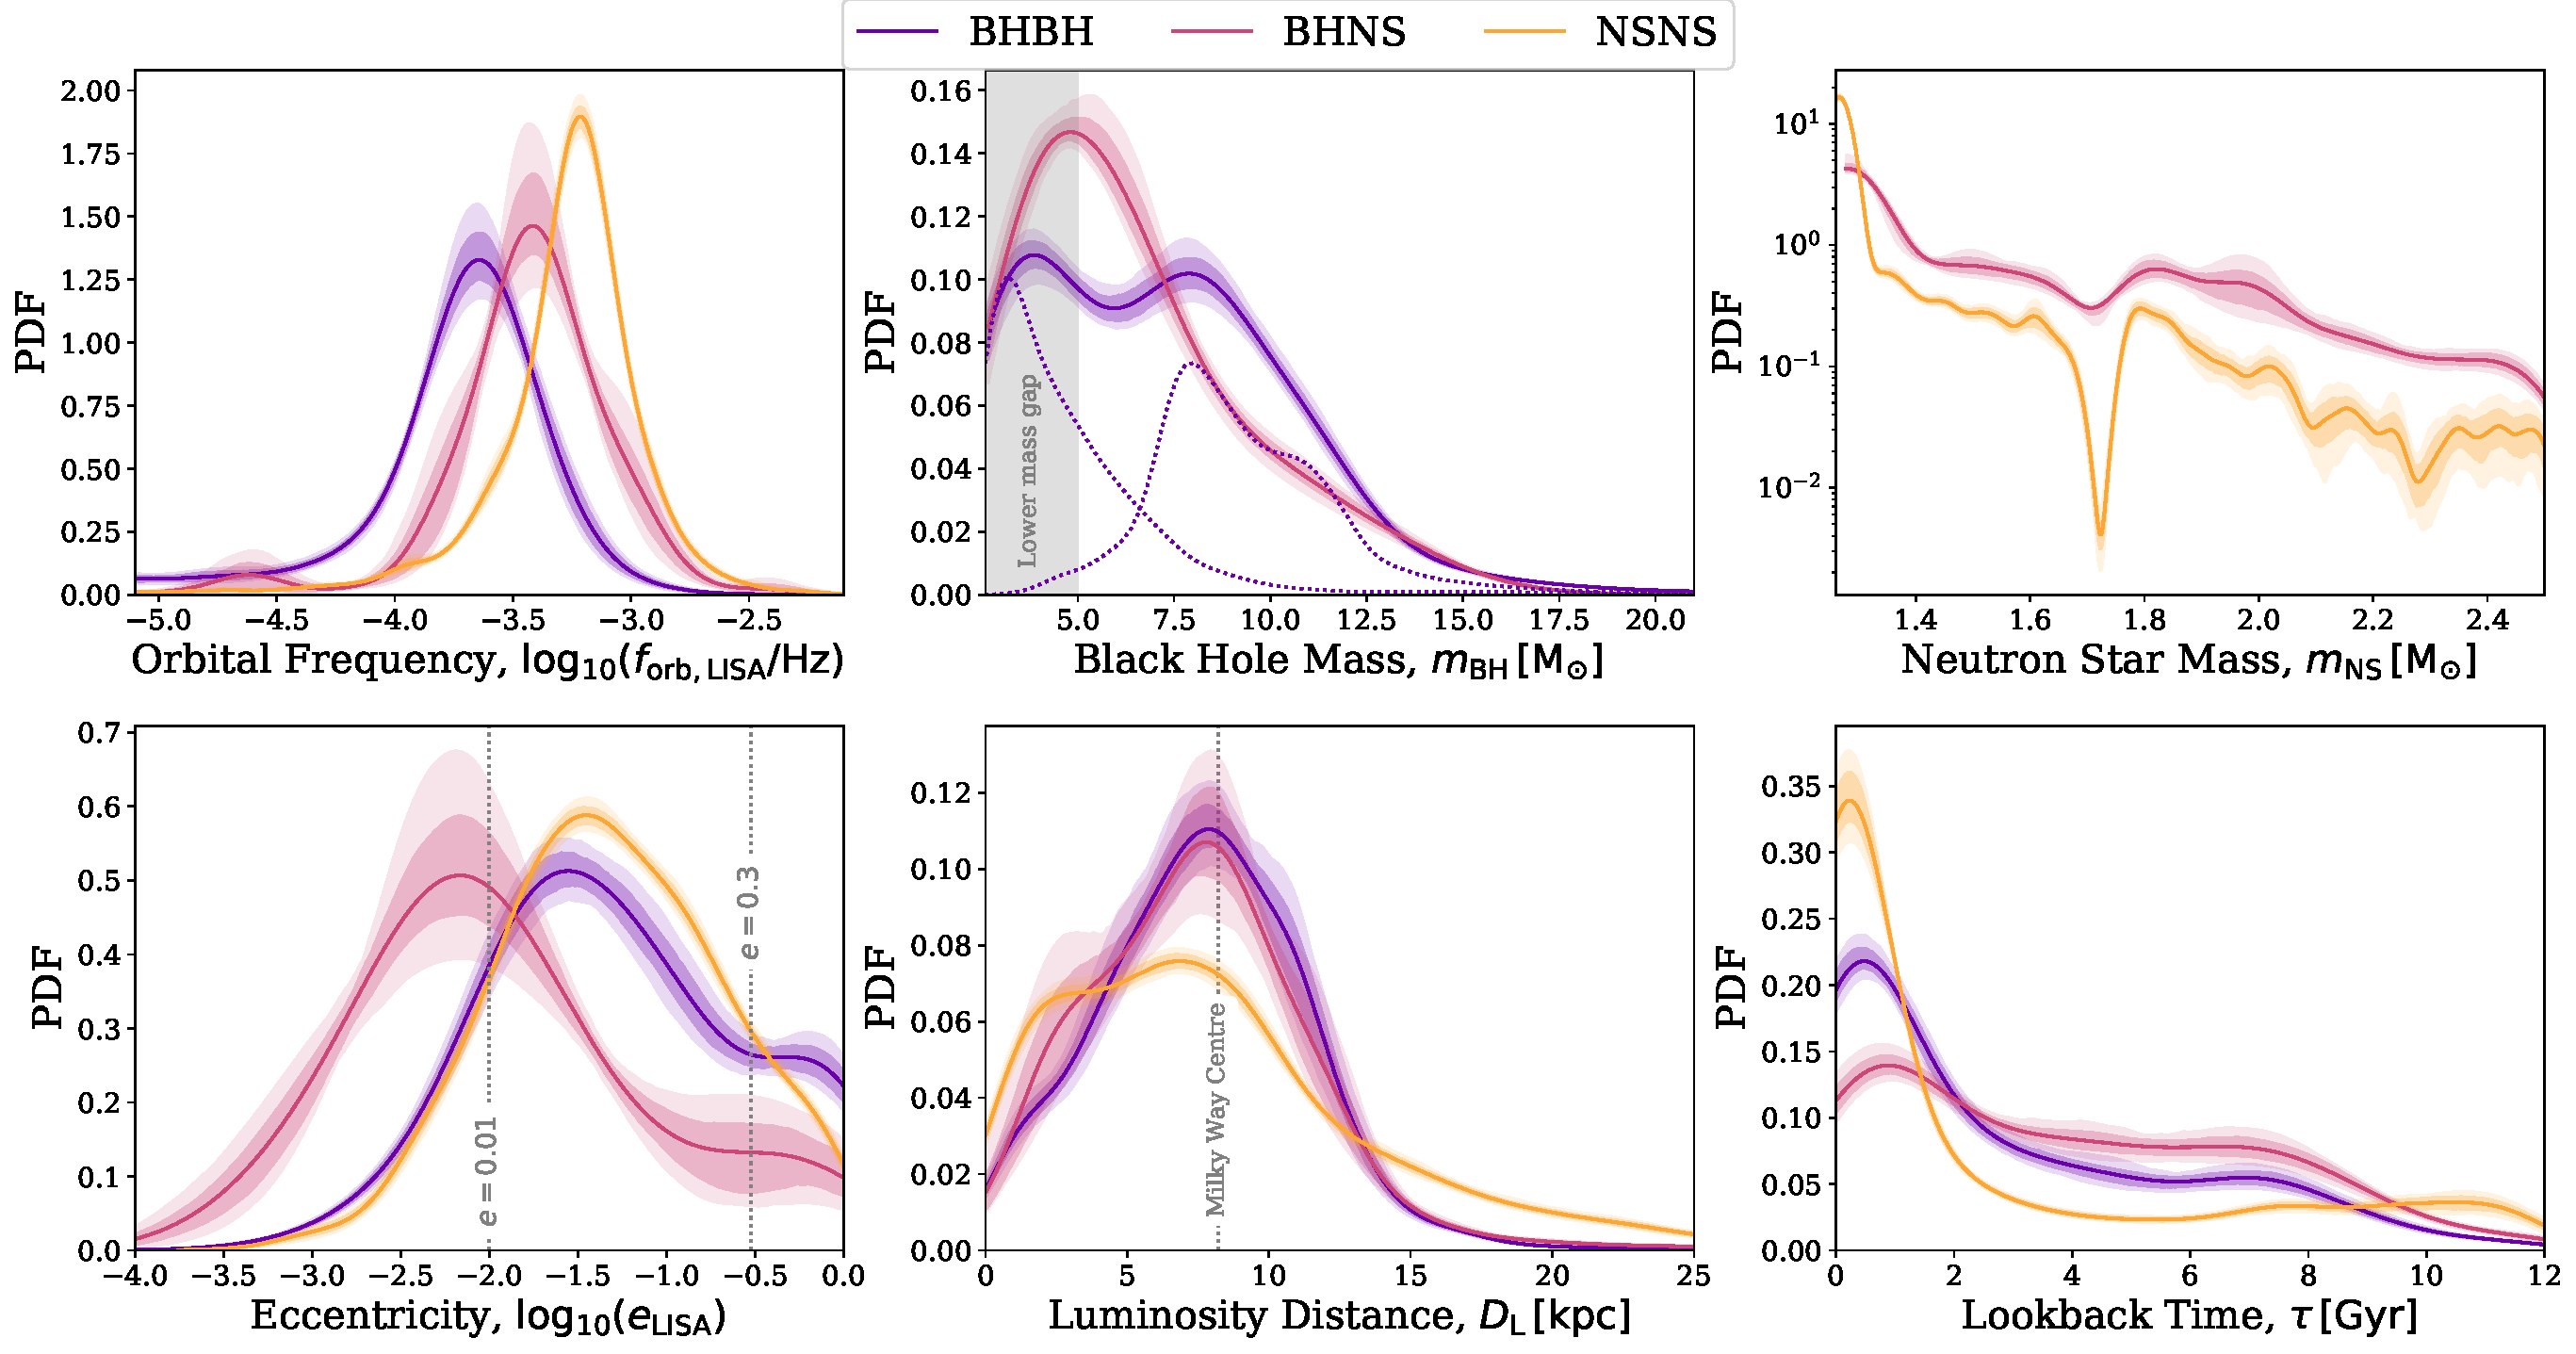
\includegraphics[width=\textwidth]{4_detectable_properties_4yr.pdf}
    \caption{Properties of detectable systems for a 4-year LISA mission in our fiducial model. Each panel shows a kernel density estimator for a single property, coloured by DCO type. The shaded areas show the 1- and 2-$\sigma$ uncertainties (obtained via bootstrapping). The dotted lines in the black hole mass panel show the individual primary and secondary mass distributions. See Sec.~\ref{sec:fiducial_distributions} for a discussion.}
    \label{fig:fiducial_pdf_distributions}
\end{figure*}

\subsubsection{Orbital Frequency}
The orbital frequency distributions for BHBHs, BHNSs and NSNSs peak at progressively increasing frequencies. This is because a higher mass DCO at the same distance and eccentricity requires a lower frequency to produce the same signal-to-noise ratio and thus be detected. The BHBH distribution has a tail that extends to $8 \times 10^{-6} \unit{Hz}$, which is comprised of highly eccentric binaries. These systems are still detectable by LISA as the high eccentricity means that the majority of the GW signal is emitted at higher harmonics at higher frequencies that are located in the LISA band. Similar tails are not as prevalent for BHNSs and NSNSs as they do not have as many eccentric binaries.

\subsubsection{Black Hole Mass}
For both the BHBHs and BHNSs, the black hole mass distribution extends across relatively low masses, with $88\%$ and $90\%$ respectively below $11 \unit{M_{\odot}}$. Unlike ground-based detector, LISA is not biased to higher masses and so the mass distribution more closely follows the IMF. In addition, at the high metallicities in the Milky Way, stellar winds are much stronger and strip away much of the stellar mass before BH formation, resulting the less massive black holes. The mass distribution extends down to $2.5 \unit{M_{\odot}}$, our fiducial maximum neutron star mass, since the \citet{Fryer+2012} \textit{delayed} remnant mass prescription does not produce a mass gap between neutron stars and black holes. Indeed we expect $35\%$ and $39\%$ of detected BHBH and BHNS systems to contain a black hole in the lower mass gap. Therefore, LISA could help to confirm or rule out the existence of the lower mass gap.

The bimodality of the BHBH distribution is a result of most detectable BHBHs in our sample having unequal mass ratios. The two peaks are from the primary and secondary black hole masses, which peak around $8 \unit{M_{\odot}}$ and $3.5 \unit{M_{\odot}}$ respectively. We show these individual distributions as dotted curves below the main BHBH distribution.

The reasoning for these unequal mass ratio systems is as follows: in order to produce a BHBH, most formation channels require at least the first mass transfer to be stable. This stability is strongly dependent on the mass ratio such that equal mass ratios (at the moment of mass transfer) are preferred for creating BHBHs. Yet, since stellar winds are so strong at high metallicity, and even stronger for more massive stars, the primary star will experience significant mass loss and so an initially \textit{unequal} mass ratio is preferred so that the masses are more balanced at the first instance of mass transfer. Since mass transfer occurs after the end of the main sequence for most of our BHBHs, the star will have a well defined core and these core masses, which go on to form BHs, will reflect the initially unequal mass ratios.

\subsubsection{Neutron Star Mass}
The neutron star mass distribution shows that most neutron stars have low masses, with $77\%$ and $91\%$ having masses below $1.7 \unit{M_{\odot}}$ for BHNSs and NSNSs respectively. The lack of neutron stars around $1.7 \unit{M_{\odot}}$ and the subsequent small peaks are artifacts of the discontinuous nature of the \citet{Fryer+2012} remnant mass prescription and do not have strong effects since the vast majority of NSs are formed with lower masses.

Both distributions have notable peaks around $1.26 \unit{M_{\odot}}$, though more strongly in the NSNS case, which are a result of the combination of two effects. Firstly, we set the remnant mass for all electron-capture supernovae to $1.26 \unit{M_\odot}$ (see Sec.~\ref{sec:fiducial_physics}) and thus this leads to a pileup when many systems are formed through ECSN. In addition, the Fryer remnant mass prescription gives a fixed fallback mass for any star with a CO core mass less than $2.5 \unit{M_\odot}$, such that many NSs are given the identical mass of $1.278 \unit{M_\odot}$ in the \textit{delayed} prescription \citep[see][Eq.~19]{Fryer+2012}. 

\subsubsection{Luminosity Distance}
Each DCO's luminosity distance distribution peaks around $8 \unit{kpc}$ since this is the distance to the centre of the Milky Way and thus the most dense location of DCOs. There is a clear bias in each distribution for systems at lower distances since closer binaries are easier to detect. This bias is most prominent for the NSNS distribution since, on average, their lower relative masses require a smaller distance in order to be detected.

\subsubsection{Lookback Time}
Although when creating each mock Milky Way galaxy the lookback time is drawn independently from other parameters, and in the same way for every DCO type, the distributions are clearly different for each type of DCO. This is because for a binary to be detectable, it must have an orbital frequency within the LISA band. Therefore a binary needs to have completed most of its inspiral to be visible in the LISA band and thus detectable systems will tend to have lookback time that are close to their merger times, which \textit{are} a function of other binary parameters.

Since most of the DCOs are formed through common envelope events, their initial separations are relatively tight and so if a binary it given a long lookback time, it will have merged before the LISA mission. This explains the peak in each distribution at short lookback times. The later lookback times correspond to systems that are formed through channels in which mass transfer is only stable and no common envelope event occurs.

The trends across the different DCO types can be explained by considering that the merger time is a function of the masses, frequency and eccentricity of th source. This dependence can be approximately written as $t_{\rm merge} \propto f_{\rm orb}^{-4} m_1^{-3} (1 - e^2)^{-7/2}$,  \citep[][Eq.~5.14]{Peters+1964}. Therefore, although NSNSs are the lowest mass systems, their relatively higher orbital frequencies means that they have the shortest merger times. This same logic implies that BHNSs should have the next shortest merger times and then BHBHs. This order is flipped due to the fact that high eccentricity results in a shorter merger time and we find that LISA detectable BHNSs are mostly circular, whilst BHBHs have a significant highly eccentric subpopulation.

\subsubsection{Eccentricity}
The eccentricity distributions show that detectable BHBHs are the most eccentric of the three DCOs. This may seem counter-intuitive since neutron stars receive stronger natal kicks, which cause the orbit to become eccentric. However, these stronger kicks often instead result in disrupted or too-wide binaries in more weakly bound NSNSs. In contrast, BHBHs can receive strong kicks that impart high eccentricity without disrupting and thus tend to be more eccentric. This effect is compounded by the fact that we can see BHBHs at lower orbital frequencies, meaning that they have not had as much time to circularise and so still have significant eccentricity by the time of the LISA mission.

A significant fraction of DCOs in each population have eccentricities greater than 0.01, the lower bound on the measurable eccentricity with LISA proposed by \citet{Nishizawa+2016}, which we indicate with the shaded area. We discuss the estimation of the eccentricity uncertainty further in Section~\ref{sec:measurement_uncertainties}

\subsection{Measurement Uncertainties}\label{sec:measurement_uncertainties}
Although it is useful to investigate the underlying parameters of the detectable population, it is also important to consider what LISA will actually \textit{measure} during a detection.

\subsubsection{Eccentricity uncertainty}\label{sec:ecc_unc}
One of the main advantage of space-based gravitational wave detectors such as LISA is that systems may still have significant eccentricity during the LISA mission. Whilst also being useful as an individual quantity for learning more about sources, the uncertainty on the eccentricity also affects the uncertainty on the chirp mass and so it is important to quantify this uncertainty.

We follow a method used in previous works that uses the individually detectable harmonics of sources to determine the uncertainty of the eccentricity of a source \citep[e.g.][]{Lau+2020, Korol+2021}. Eccentric sources emit at several evenly spaced harmonic frequencies, each with a different fraction of the gravitational wave power and the distribution of the power over the harmonics changes with eccentricity. Therefore, by measuring the SNR of each individual harmonic and finding the ratio of the SNR of the two most detectable harmonics that are above the detection threshold, one can determine the eccentricity. The uncertainty on the eccentricity can therefore be written as a combination of the uncertainty on the SNR of the two most detectable harmonics. In the limit of large SNRs, the eccentricity uncertainty, $\Delta e$, can be written as 
\begin{equation}
    \Delta e = \frac{1}{\rho_1} + \frac{1}{\rho_2},
\end{equation}
where $\rho_1$ and $\rho_2$ are the SNRs of the two most detectable harmonics.

In some cases, sources may only have one individually detectable harmonic, or even none. In these cases one can only put a lower or upper bound on the eccentricity. For sources with only one detectable harmonic, the source is either a circular source or a source with a small enough eccentricity that most of the GW power is still concentrated in the $n = 2$ harmonic. Therefore, we can use this information to place an upper bound on the eccentricity. Conversely, sources with no detectable harmonics must be eccentric enough such that the GW power has spread over so many harmonics that no single harmonic has a significantly stronger signal. Therefore, we can use this information to place a lower bound on the eccentricity.

This method provides a pessimistic estimate of the eccentricity of sources since we do not consider the benefits of any sort of matched-filter analysis or similar methods.

\subsubsection{Chirp mass uncertainty}
The chirp mass uncertainty can be calculated using the uncertainty on the orbital frequency, the time derivative of the orbital frequency and the eccentricity. This is because the time derivative of the orbital frequency can be written as
\begin{equation}\label{eq:f_n_dot}
    \dot{f}_{n} = \frac{48 n}{5 \pi} \frac{(G \mathcal{M}_c)^{5/3}}{c^3} (2 \pi f_{\rm orb})^{11/3} F(e),
\end{equation}
where $f_{\rm orb}$ is the orbital frequency, $\mathcal{M}_{c}$ is the chirp mass (defined in Eq.~\ref{eq:chirp_mass}) and $e$ is the eccentricity and
\begin{equation}
    F(e) = \frac{1 + \frac{73}{24} e^2 + \frac{37}{96} e^4}{(1 - e^2)^{7/2}},
\end{equation}
is the enhancement factor of gravitational wave emission for an eccentric binary over an otherwise identical circular binary \citep[][Eq.~17]{Peters+1963}.

We can invert this and instead write that the chirp mass is
\begin{equation}
    \mathcal{M}_c = \frac{c^3}{G} \left( \frac{5 \pi}{48 n} \frac{\dot{f}_{n}}{F(e)} \right)^{3/5} \frac{1}{(2 \pi f_{\rm orb})^{11/5}},
\end{equation}
and therefore that the chirp mass uncertainty is
\begin{equation}\label{eq:chirp_mass_uncertainty}
    \qty( \frac{\Delta \mathcal{M}_c}{\mathcal{M}_c} )^2 = \left( \frac{11}{5} \frac{\Delta f_{\rm orb}}{f_{\rm orb}} \right)^2 + \left( \frac{3}{5} \frac{\Delta \dot{f}_{\rm dom}}{\dot{f}_{\rm dom}} \right)^2 + \left( \frac{3}{5} \frac{\Delta F(e)}{F(e)} \right)^2,
\end{equation}
where $f_{\rm dom}$ is the harmonic frequency with the strongest SNR as this will provide the best measurement.

We calculate the frequency uncertainties using \citet{Takahashi+2002}, such that
\begin{align}\label{eq:f_orb_unc}
    \frac{\Delta f_{\rm orb}}{f_{\rm orb}} &= 4 \sqrt{3} \cdot \frac{1}{\rho} \frac{1}{T_{\rm obs}} \frac{1}{f_{\rm orb}}, \\
    \frac{\Delta \dot{f}_{\rm dom}}{\dot{f}_{\rm dom}} &= 6 \sqrt{5} \cdot \frac{1}{\rho} \left(\frac{1}{T_{\rm obs}} \right)^2 \frac{1}{\dot{f}_{\rm dom}},
\end{align}
where $\rho$ is the signal-to-noise ratio and $T_{\rm obs}$ is the LISA mission length. Then we calculate the eccentricity certainty, $\Delta e$, as discussed in Sec.~\ref{sec:ecc_unc} and propagate it so that
\begin{equation}
    \frac{\Delta F(e)}{F(e)} = \Delta e \cdot \frac{(1256 + 1608 e^2 + 111 e^4) e}{96 + 196 e^2 - 255 e^4 - 37 e^6}.
\end{equation}

We use Eq.~\ref{eq:chirp_mass_uncertainty} to calculate the chirp mass uncertainty for each DCO in our sample and plot it in the lower centre panel of Fig.~\ref{fig:fiducial_pdf_distributions}. We show the distribution as a CDF that is normalised to the expected number of detections to better indicate the absolute number of detections that will have well determined chirp masses. We find that approximately 10 BHBHs, 10 BHNSs and 5 NSNSs have measurable chirp masses (as indicated by the shaded region). This uncertainty is generally dominated by the uncertainty on the time derivative of the frequency since most of the binaries are too early in their inspiral for LISA to measure a strong chirp.

\subsubsection{Sky localisation}
We quantify the sky localisation of a source by calculating its angular resolution. Since we find that all potential sources are stationary on the timescale of the LISA mission, following \citet{Mandel+2018}, we can use the timing accuracy of LISA and the effective detector baseline to calculate the angular resolution, $\sigma_{\theta}$, as
\begin{equation}
    \sigma_{\theta} = 16.6^\circ \left(\frac{7}{\rho}\right) \left(\frac{5 \times 10^{-4} \unit{Hz}}{f_{\rm dom}}\right) \left( \frac{2 \unit{AU}}{L} \right),
\end{equation}
where $\rho$ is the signal-to-noise ratio, $f_{\rm dom}$ is the harmonic frequency with the strongest signal-to-noise ratio ($f_{\rm dom} = n_{\rm dom} f_{\rm orb}$ and $n_{\rm dom} = 2$ for circular binaries) and $L$ is the effective detector baseline.

We plot the angular resolution in the last panel of Fig.~\ref{fig:fiducial_pdf_distributions} as a CDF normalised to the expected detection rate of each DCO. From this plot, we see that the majority of sources can be resolved to an angular resolution of 10 square degrees. The size of a pencil beam for a 15m diameter SKA dish observing at 1.4 GHz is roughly 0.67 square degrees, corresponding to an angular resolution of $\sigma_\theta = \sqrt{(0.67 / \pi)} = 0.46^\circ$ (which, for intuition, is approximately the angular size of the moon). Applying this to the plot shows that about 20\% of DCOs can be covered by a single pointing of SKA. We will discuss the prospects of matching LISA detections to radio pulsars with SKA further in Sec.~\ref{sec:pulsar_matching}.

\subsection{Model variations}
\tom{This will be about how the shapes of the parameter distributions change for the different model variations. I won't detail every variation but I'll point out anything that stands out and leave the rest in the appendix plots.}